\documentclass[english]{article}
\usepackage[T1]{fontenc}
\usepackage[latin9]{inputenc}
\usepackage[a4paper]{geometry}
\usepackage{amsmath}
\geometry{verbose,tmargin=2cm,bmargin=2cm,lmargin=2cm,rmargin=2cm}
\usepackage{graphicx}
\usepackage{algorithm}
\usepackage{algpseudocode}
\usepackage{pifont}
\usepackage{courier}

\usepackage{color}
\usepackage{listings}
\usepackage{setspace}
\definecolor{Code}{rgb}{0,0,0}
\definecolor{Decorators}{rgb}{0.5,0.5,0.5}
\definecolor{Numbers}{rgb}{0.5,0,0}
\definecolor{MatchingBrackets}{rgb}{0.25,0.5,0.5}
\definecolor{Keywords}{rgb}{0,0,1}
\definecolor{self}{rgb}{0,0,0}
\definecolor{Strings}{rgb}{0,0.63,0}
\definecolor{Comments}{rgb}{0,0.63,1}
\definecolor{Backquotes}{rgb}{0,0,0}
\definecolor{Classname}{rgb}{0,0,0}
\definecolor{FunctionName}{rgb}{0,0,0}
\definecolor{Operators}{rgb}{0,0,0}
\definecolor{Background}{rgb}{0.98,0.98,0.98}
\lstdefinelanguage{Python}{
numbers=left,
numberstyle=\footnotesize,
numbersep=1em,
xleftmargin=1em,
framextopmargin=2em,
framexbottommargin=2em,
showspaces=false,
showtabs=false,
showstringspaces=false,
frame=l,
tabsize=4,
% Basic
basicstyle=\ttfamily\small\setstretch{1},
backgroundcolor=\color{Background},
% Comments
commentstyle=\color{Comments}\slshape,
% Strings
stringstyle=\color{Strings},
morecomment=[s][\color{Strings}]{"""}{"""},
morecomment=[s][\color{Strings}]{'''}{'''},
% keywords
morekeywords={import,from,class,def,for,while,if,is,in,elif,else,not,and,or,print,break,continue,return,True,False,None,access,as,,del,except,exec,finally,global,import,lambda,pass,print,raise,try,assert},
keywordstyle={\color{Keywords}\bfseries},
% additional keywords
morekeywords={[2]@invariant,pylab,numpy,np,scipy},
keywordstyle={[2]\color{Decorators}\slshape},
emph={self},
emphstyle={\color{self}\slshape},
%
}
\linespread{1.3}
\lstset{
  language=Python,                % choose the language of the code
  %numbers=left,                   % where to put the line-numbers
  stepnumber=1,                   % the step between two line-numbers.        
  numbersep=5pt,                  % how far the line-numbers are from the code % choose the background color. You must add \usepackage{color}
  showspaces=false,               % show spaces adding particular underscores
  showstringspaces=false,         % underline spaces within strings
  showtabs=false,                 % show tabs within strings adding particular underscores
  tabsize=2,                      % sets default tabsize to 2 spaces
  captionpos=b,                   % sets the caption-position to bottom
  breaklines=true,                % sets automatic line breaking
  breakatwhitespace=true,         % sets if automatic breaks should only happen at whitespace
  title=\lstname, 
  basicstyle=\footnotesize\ttfamily,                % show the filename of files included with \lstinputlisting;
}

\DeclareMathOperator*{\argmin}{\arg\!\min}
\DeclareMathOperator*{\argmax}{\arg\!\max}

\makeatletter
\def\BState{\State\hskip-\ALG@thistlm}
\providecommand{\tabularnewline}{\\}

\makeatother


\usepackage{babel}
\begin{document}

\title{\textbf{CS6700 : Reinforcement Learning } \\ Programming Assignment 1 }

\author{Akshit Kumar \\ \emph{EE14B127}}

\date{24th February 2017}

\maketitle
\tableofcontents{}

\section{Introduction}

\subsection{Goal}

The goal of this assignment is to evaluate differenet bandit algorithms on an N-armed bandit testbed. This report analyses and presents the results obtained by simulating an N-armed bandit problem on 3 types of Action-Value Methods:
\begin{itemize}
	\item $\epsilon$-greedy 
	\item Sampling from softmax distribution
	\item UCB-1 Algorithm
\end{itemize}
Each of the above algorithms are first run on a test-bed of 10-armed bandits with the results averaged over 2000 different bandit problems for 1000 time steps. In addition to this, we also compare the three algoritms on a test-bed of 1000 arms and see how the algorithm performs for the three algorithms perform by testing it on different time-steps.


\subsection{Implementation Details}
\subsubsection{True Expected Payoff of Arms}
For the purposes of experimental analysis, the true expected payoff of the arms for different bandit problems is sampled from a standard normal distribution offset by a true reward value. Therefore the true expected payoff for each arm is 
$$ q_{*}(a) = True Reward + \mathcal{N}(0,1)$$
\subsubsection{Initialization of Estimates of Expectation of Arms}
Initially all the estimates of the expectation of arms is set to zero. Therefore we have 
$$ Q_{0}(a) = 0 \hspace{10 mm} \forall a \in \mathcal{A} $$ 
\subsubsection{Sampling of Rewards for Arms}
The rewards for each of the arms at each time step in each of the bandit problems is sampled from a standard normal distribution offset by the true expected payoff of that arm. Therefore we have
$$ R_{i} = q_{*}(a) + \mathcal{N}(0,1) $$ where $R_{i}$ is the reward at time step $i$ and $\mathcal{N}(0,1)$ adds noise to the true expected payoff for that action.
\subsubsection{Update of the Estimate of Arms}
For updating the estimates of the arm, incremental updates are made and the update equation is given as
$$ Q_{t+1} = Q_{t} + \dfrac{1}{t}[R_{t} - Q_{t}]$$

\section{Action-Value Algorithms}
In this section we discuss the algorithms of the 3 types of action-value methods mentioned above.
\subsection{$\epsilon$-Greedy}
\begin{algorithm}[H]
\caption{$\epsilon$-greedy Algorithm}
\label{EGAlgorithm}
\begin{algorithmic}[1]
\Procedure{$\epsilon$-Greedy Procedure}{}
\For{each action $a$ \Pisymbol{psy}{206} $\mathcal{A}$ }
\State Q(a)$\leftarrow$0
\State N(a) $\leftarrow$ 0
\EndFor
\Loop
	\If {sample from $\mathcal{N}(0,1) > \epsilon$}
		\State $\mathcal{A} \leftarrow \argmax_{a} Q(a)$
	\Else 
		\State $\mathcal{A} \leftarrow$ randint(0,\# of arms)
	\EndIf
	\State $\mathcal{R} \leftarrow getReward(\mathcal{A})$
	\State $N(\mathcal{A}) \leftarrow N(\mathcal{A}) + 1$
	\State $Q(\mathcal{A}) \leftarrow Q(\mathcal{A}) + \dfrac{1}{N(A)}[R - Q(A)]$
\EndLoop
\EndProcedure
\end{algorithmic}
\end{algorithm}
This algorithm introduces some randomness in selection of action to take at step $t+1$ which allows us to explore more actions and not settle for a suboptimal arm. At each step, with probability $\epsilon$ , a random exploratory move is played and with probability $1 - \epsilon$, a greedy action selection is made based on the current estimates of the expectation of the arms.

\subsection{Sampling from softmax distribution}
\begin{algorithm}[H]
\caption{Sampling from Softmax Distribution}
\label{SoftmaxAlgorithm}
\begin{algorithmic}[2]
\Procedure{Sampling from Softmax Distribution}{}
\For{each action $a$ \Pisymbol{psy}{206} $\mathcal{A}$ }
\State Q(a) $\leftarrow$ 0
\State N(a) $\leftarrow$ 0
\EndFor
\Loop
	\State $\mathcal{A} \sim \{\dfrac{e^{Q_{t}(a_{i})/\tau}}{\sum_{a}e^{Q_{t}(a)/\tau}}\}$
	\State $\mathcal{R} \leftarrow getReward(\mathcal{A})$
	\State $N(\mathcal{A}) \leftarrow N(\mathcal{A}) + 1$
	\State $Q(A) \leftarrow Q(A) + \dfrac{1}{N(A)}[R - Q(A)]$
\EndLoop
\EndProcedure
\end{algorithmic}
\end{algorithm}
In this algorithm, we sample from a softmax distribution which is given by $$ P_{t} = \dfrac{e^{Q_{t}(a_{i})/\tau}}{\sum_{a}e^{Q_{t}(a)/\tau}} $$ where $\tau$ is the temperature parameter.

\subsection{Upper Confidence Bound}
\begin{algorithm}[H]
\caption{Upper Confidence Bound}
\label{UCBAlgorithm}
\begin{algorithmic}[1]
\Procedure{UCB-1}{}
\For{each action $a$ \Pisymbol{psy}{206} $\mathcal{A}$ }
\State play action $a$
\State $\mathcal{R} \leftarrow getReward(\mathcal{A})$
\State $Q(a) \leftarrow \mathcal{R}$
\EndFor
\Loop
	\State $\mathcal{A} \leftarrow \argmax_{a} Q(a) + \sqrt{\dfrac{2lnN}{T_{i}(n)}}$
	\State $\mathcal{R} \leftarrow getReward(\mathcal{A})$
	\State $N(\mathcal{A}) \leftarrow N(\mathcal{A}) + 1$
	\State $Q(A) \leftarrow Q(A) + \dfrac{1}{N(A)}[R - Q(A)]$
\EndLoop
\EndProcedure
\end{algorithmic}
\end{algorithm}
In this algorithm, we initially play all the actions once and then we take the subsequent actions in the remaining timesteps by being greedy with respect to the upper confidence bound on the current estimates of the actions. Therefore at each time step we choose,
$$ a = \argmax_{a} Q(a) + \sqrt{\dfrac{2lnN}{T_{i}(N)}} $$

\section{Experimental Results}
\subsection{Plots for $\epsilon$-greedy Action Selection for 10 arms}
\begin{figure}[H]
  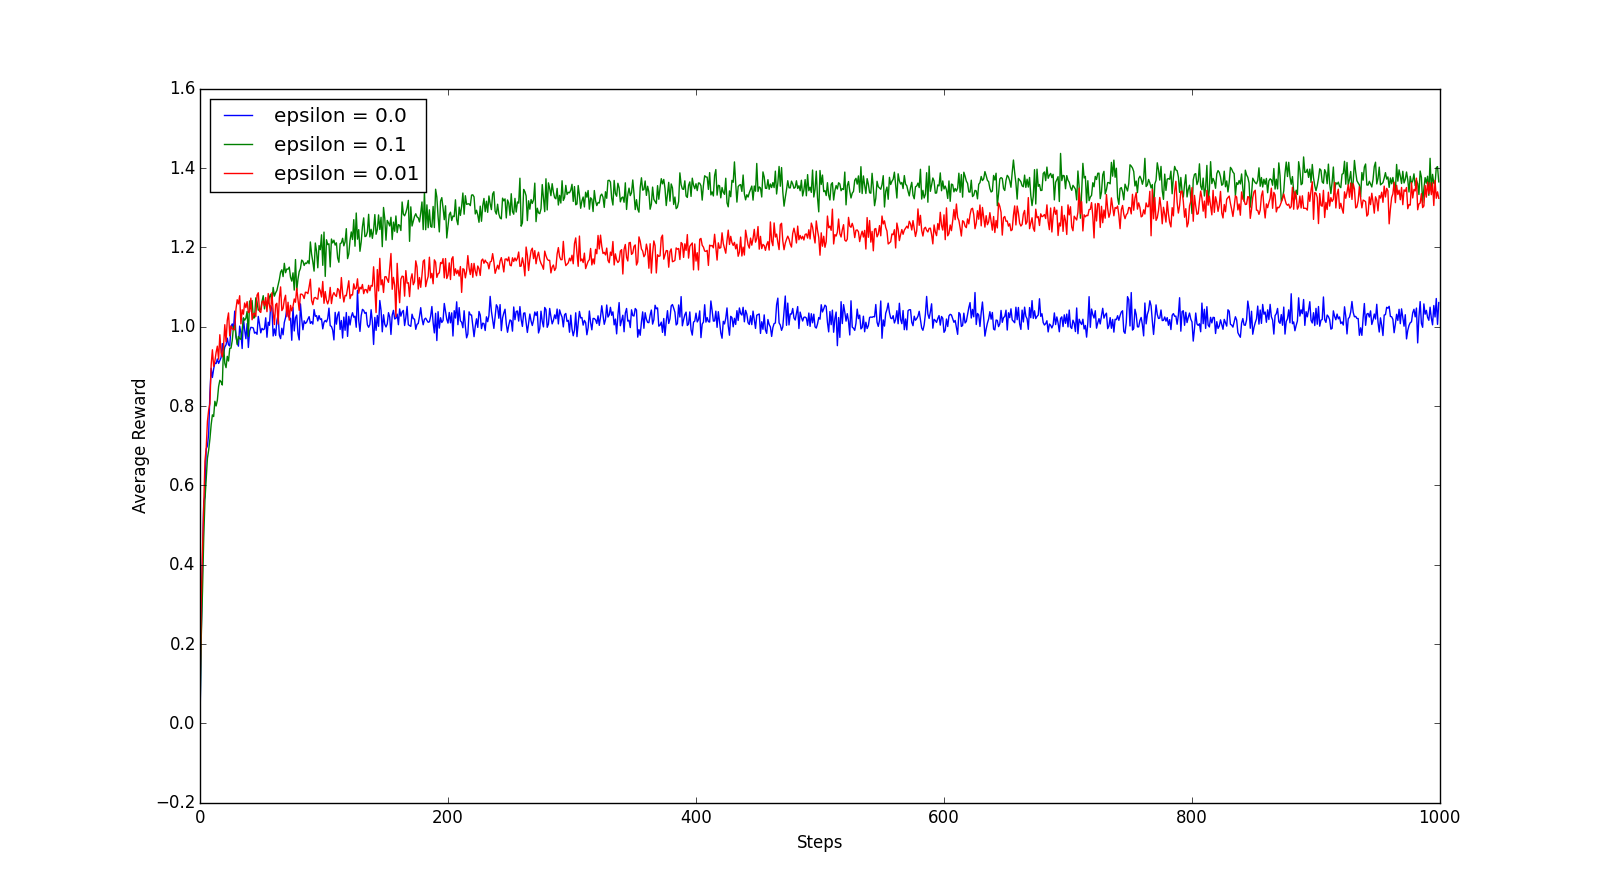
\includegraphics[width=\linewidth]{epsilon_greedy_average_reward.png}
  \caption{Plot of average reward of $\epsilon$-greedy action-value methods on the 10-armed testbed. These data are averages over 2000 runs with different bandit problems.}
  \label{fig:eg1}
\end{figure}

\begin{figure}[H]
  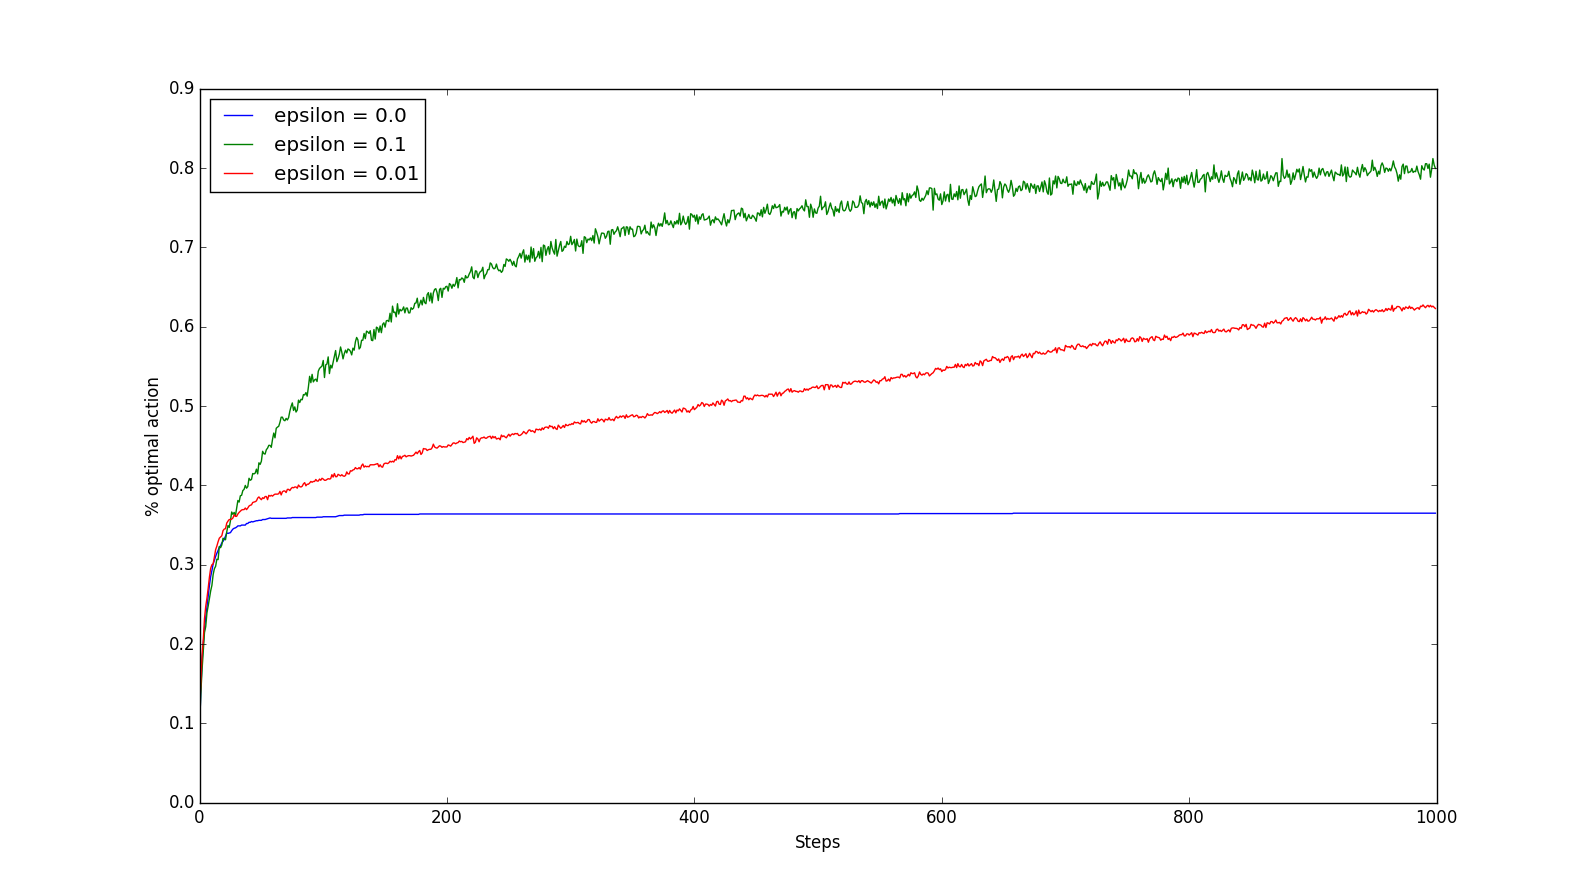
\includegraphics[width=\linewidth]{epsilon_greedy_optimal_action.png}
  \caption{Plot of \% of optimal action selection of $\epsilon$-greedy action-value methods on the 10-armed testbed. These data are averages over 2000 runs with different bandit problems.}
  \label{fig:eg1}
\end{figure}

\subsection{Plots for Softmax Action Selection for 10 arms}
\begin{figure}[H]
  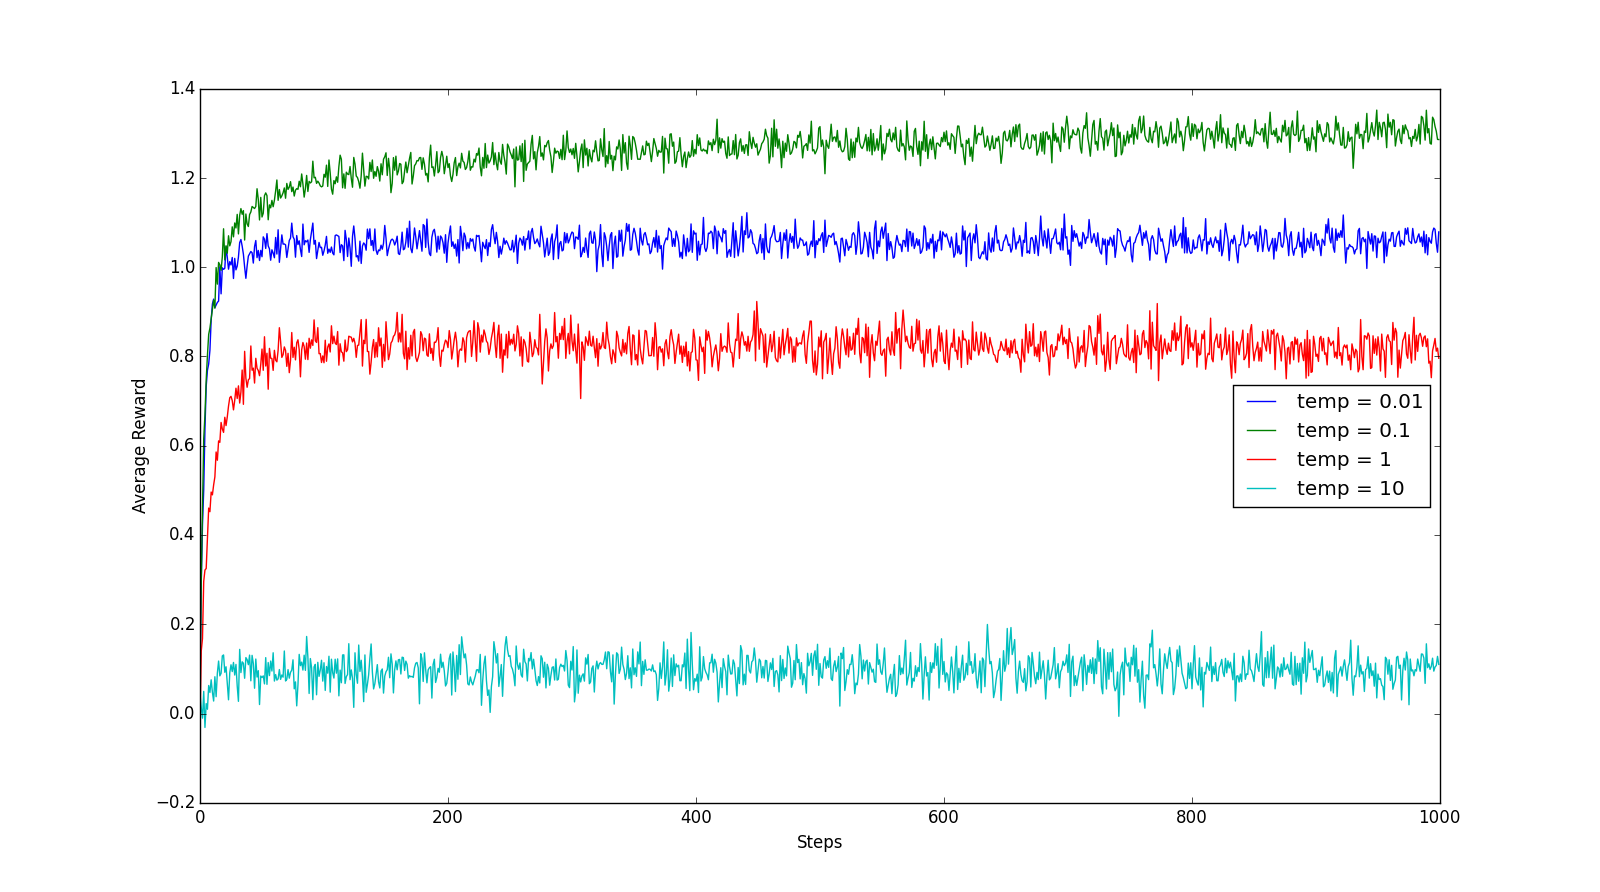
\includegraphics[width=\linewidth]{softmax_average_reward.png}
  \caption{Plot of average reward of softmax action selection methods on the 10-armed testbed. These data are averages over 2000 runs with different bandit problems.}
  \label{fig:eg1}
\end{figure}

\begin{figure}[H]
  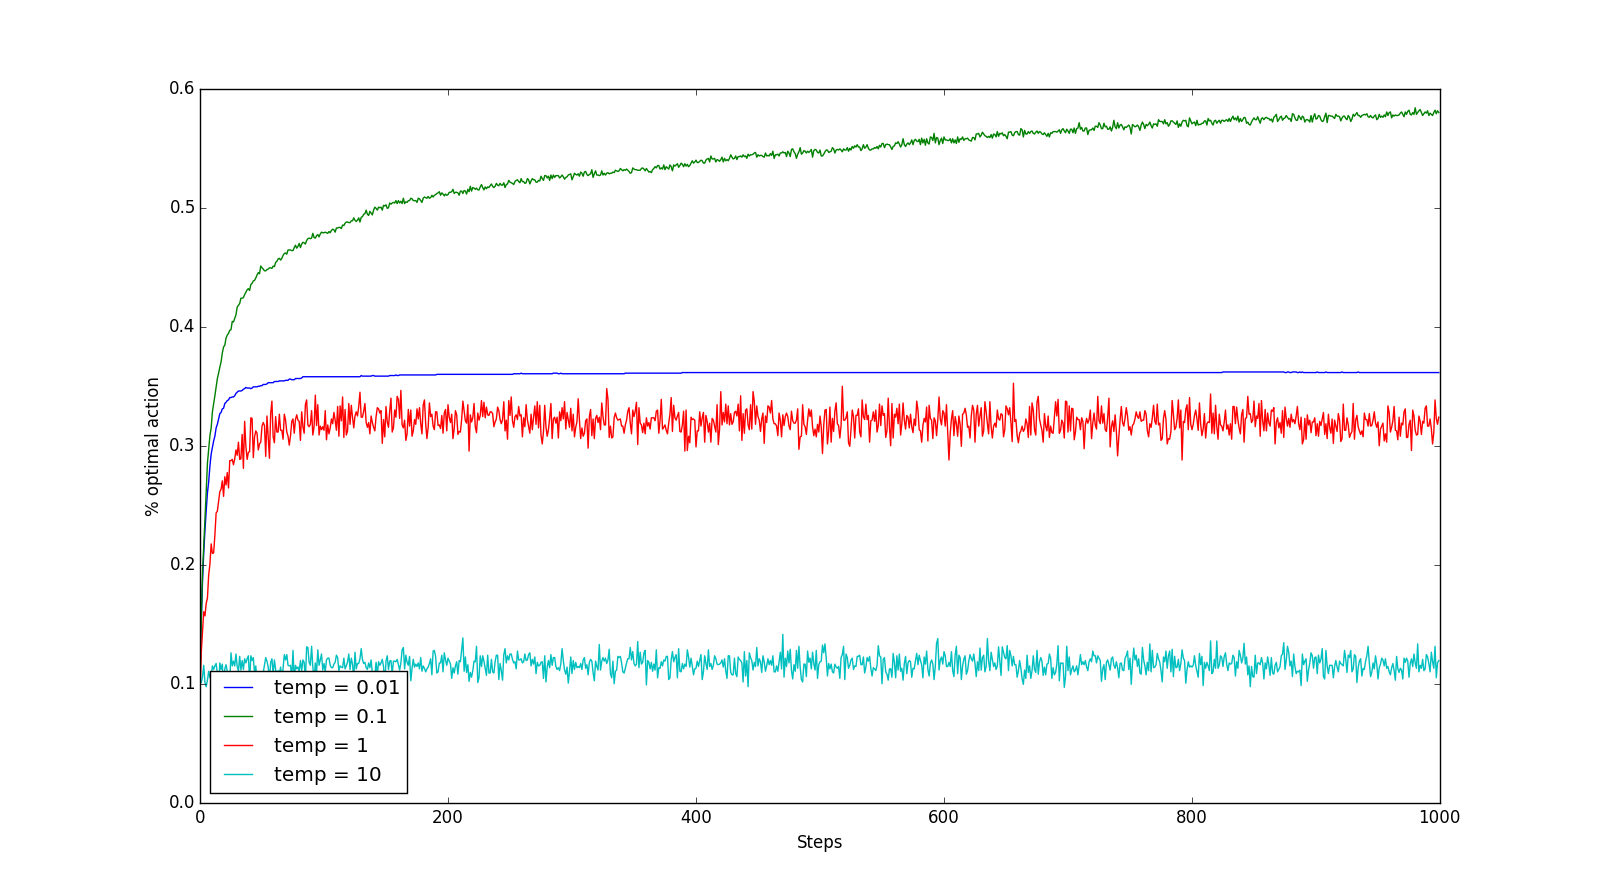
\includegraphics[width=\linewidth]{softmax_optimal_action.png}
  \caption{Plot of average reward of softmax action selection methods on the 10-armed testbed. These data are averages over 2000 runs with different bandit problems.}
  \label{fig:eg1}
\end{figure}

\subsection{Plots for UCB vs $\epsilon$-greedy vs Softmax Action Selection for 10 arms}
\begin{figure}[H]
  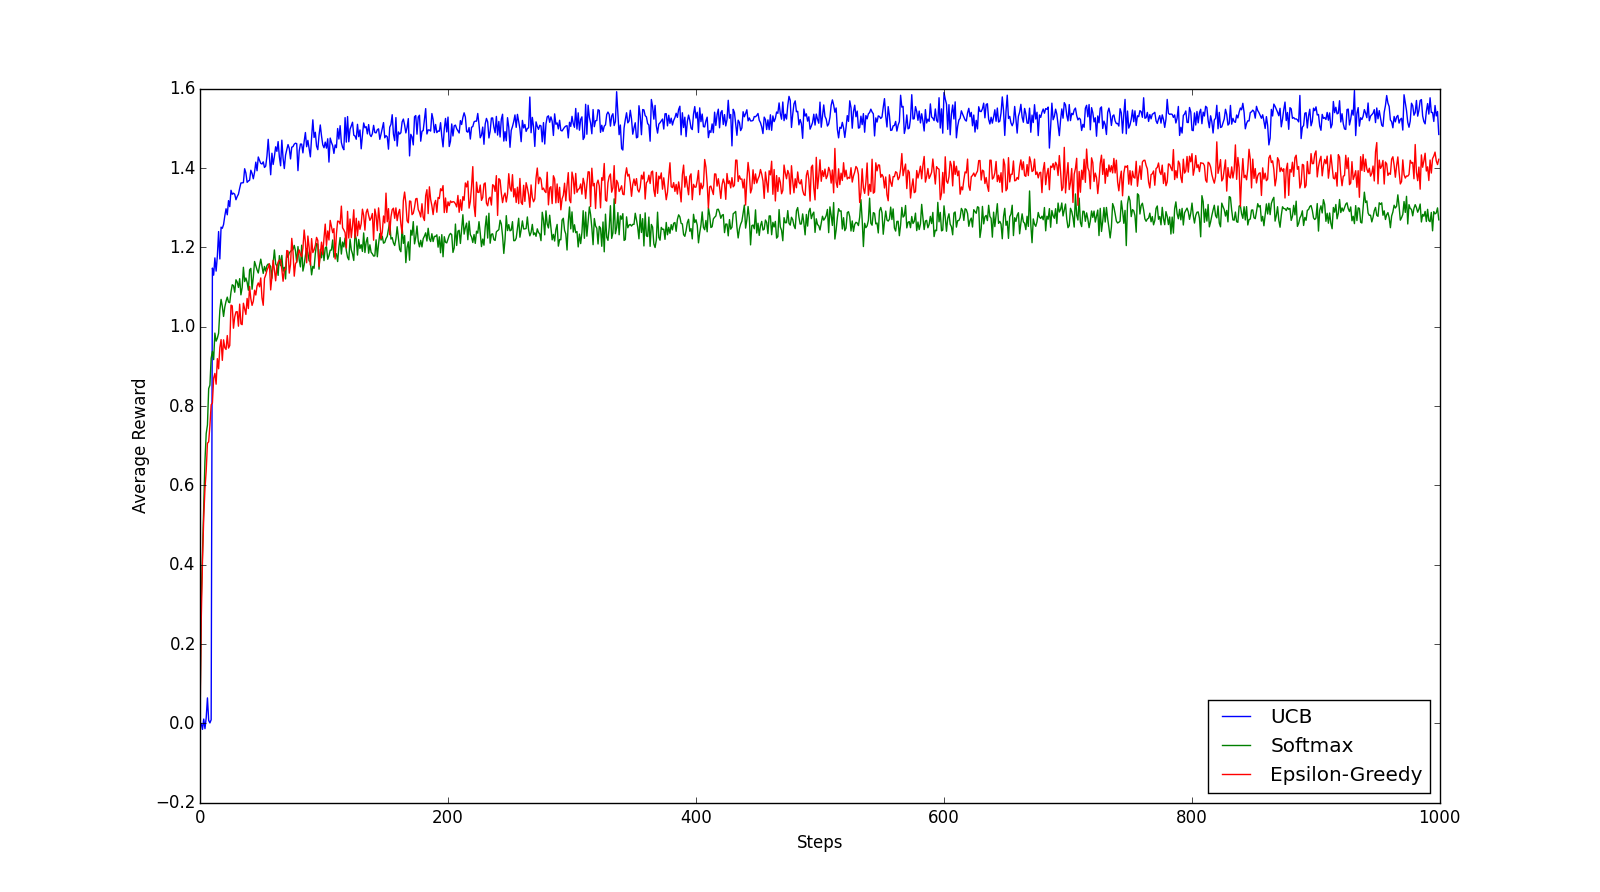
\includegraphics[width=\linewidth]{compare_ucb_10_arms_average_reward.png}
  \caption{Plot comparing the average reward accrued using UCB, $\epsilon$-greedy and Softmax Action Selection on the 10-armed testbed over 1000 timesteps. These data are averaged over 2000 runs of different bandit problems. For $\epsilon$-greedy approach, $\epsilon = 0.1 $ and for softmax action selection, $\tau = 0.1$ where $\tau$ is the temperature parameter.}
  \label{fig:eg1}
\end{figure}

\begin{figure}[H]
  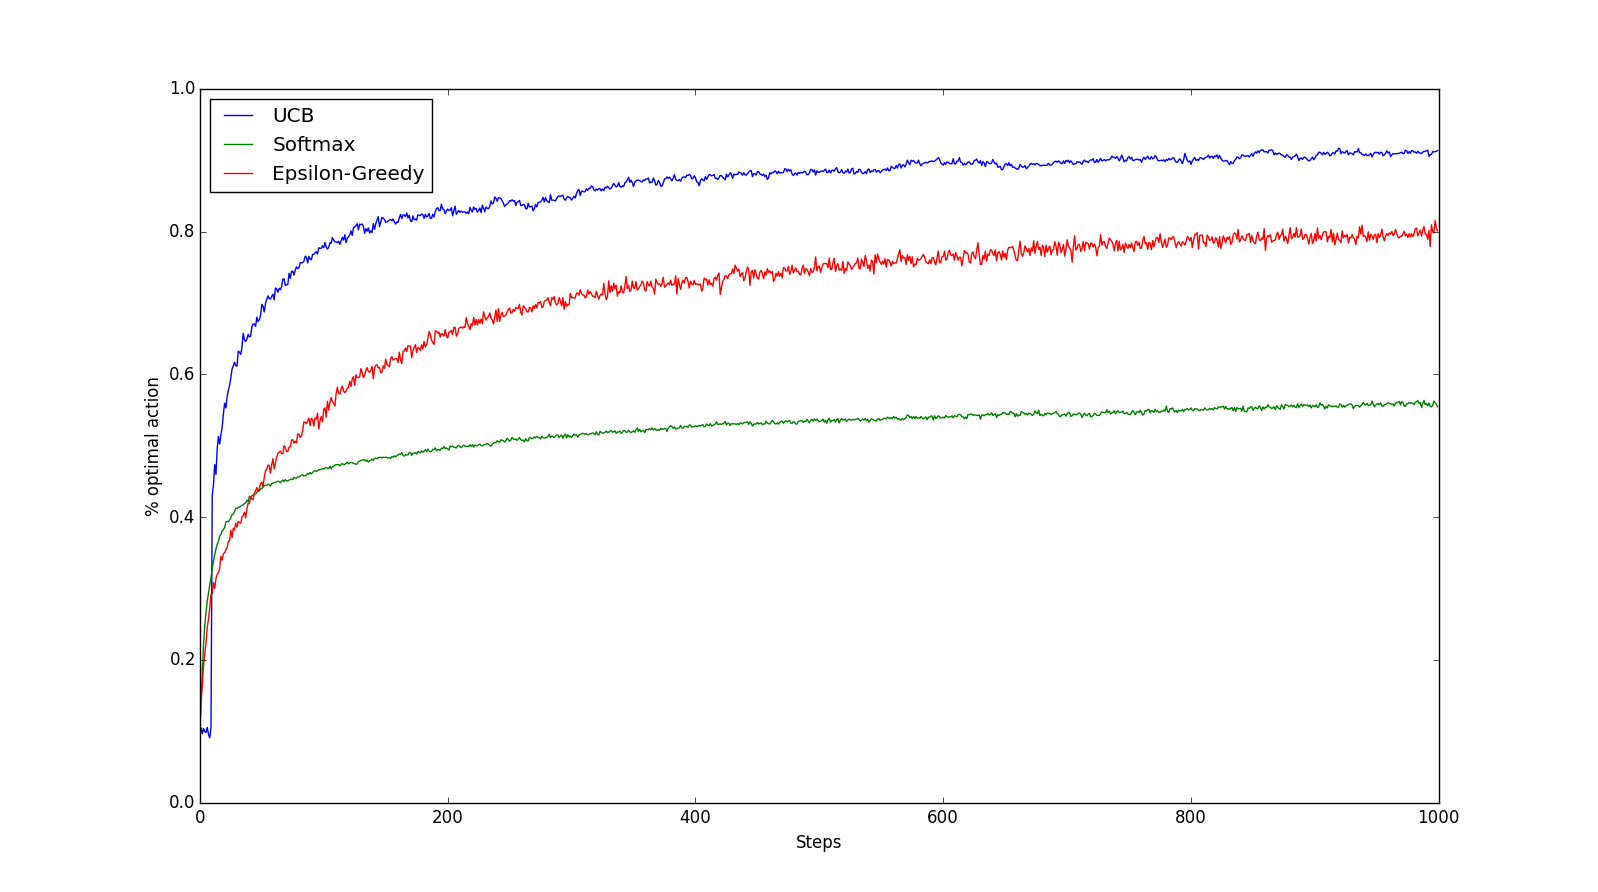
\includegraphics[width=\linewidth]{compare_ucb_10_arms_optimal_action.png}
  \caption{Plot comparing the \% optimal action selection using UCB, $\epsilon$-greedy and Softmax Action Selection on the 10-armed testbed over 1000 timesteps. These data are averaged over 2000 runs of different bandit problems. For $\epsilon$-greedy approach, $\epsilon = 0.1 $ and for softmax action selection, $\tau = 0.1$ where $\tau$ is the temperature parameter.}
  \label{fig:eg1}
\end{figure}

\subsection{Plots for UCB vs $\epsilon$-greedy vs Softmax Action Selection for 1000-arms}
\subsubsection{Plots for 1000 time-steps}
\begin{figure}[H]
  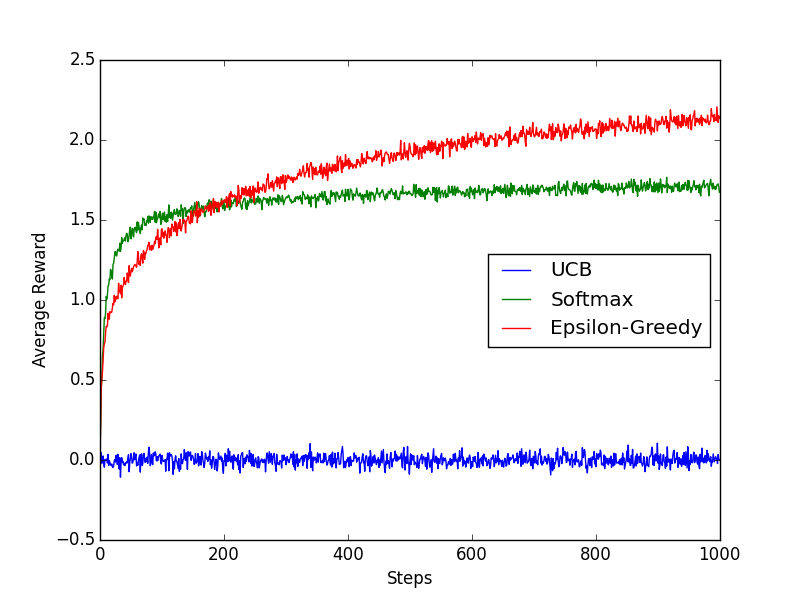
\includegraphics[width=\linewidth]{compare_ucb_1000_arms_1000_steps_average_reward.png}
  \caption{Plot comparing the average reward accrued using UCB, $\epsilon$-greedy and Softmax Action Selection on the 1000-armed testbed over 1000 timesteps. These data are averaged over 2000 runs of different bandit problems. For $\epsilon$-greedy approach, $\epsilon = 0.1 $ and for softmax action selection, $\tau = 0.1$ where $\tau$ is the temperature parameter.}
  \label{fig:eg1}
\end{figure}

\begin{figure}[H]
  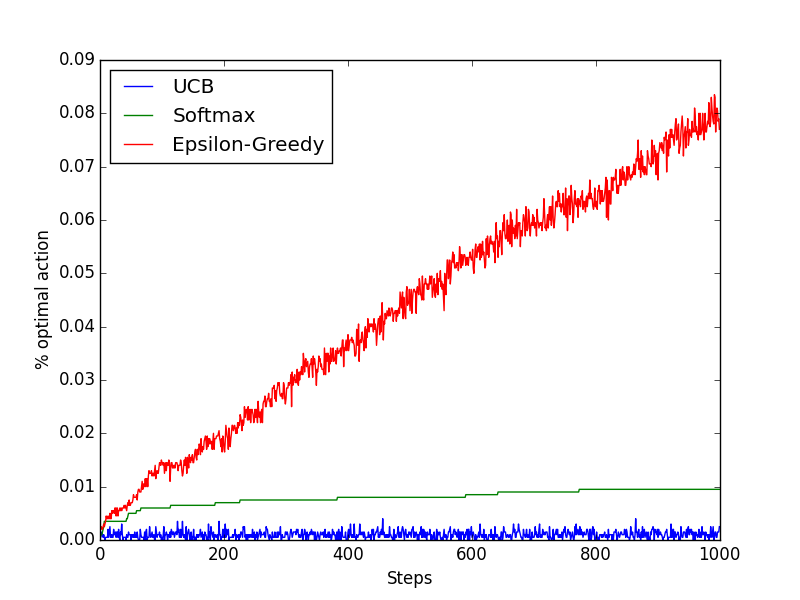
\includegraphics[width=\linewidth]{compare_ucb_1000_arms_1000_steps_optimal_action.png}
  \caption{Plot comparing the average reward accrued using UCB, $\epsilon$-greedy and Softmax Action Selection on the 1000-armed testbed over 1000 timesteps. These data are averaged over 2000 runs of different bandit problems. For $\epsilon$-greedy approach, $\epsilon = 0.1 $ and for softmax action selection, $\tau = 0.1$ where $\tau$ is the temperature parameter.}
  \label{fig:eg1}
\end{figure}

\subsubsection{Plots for 10000 time-steps}
\begin{figure}[H]
  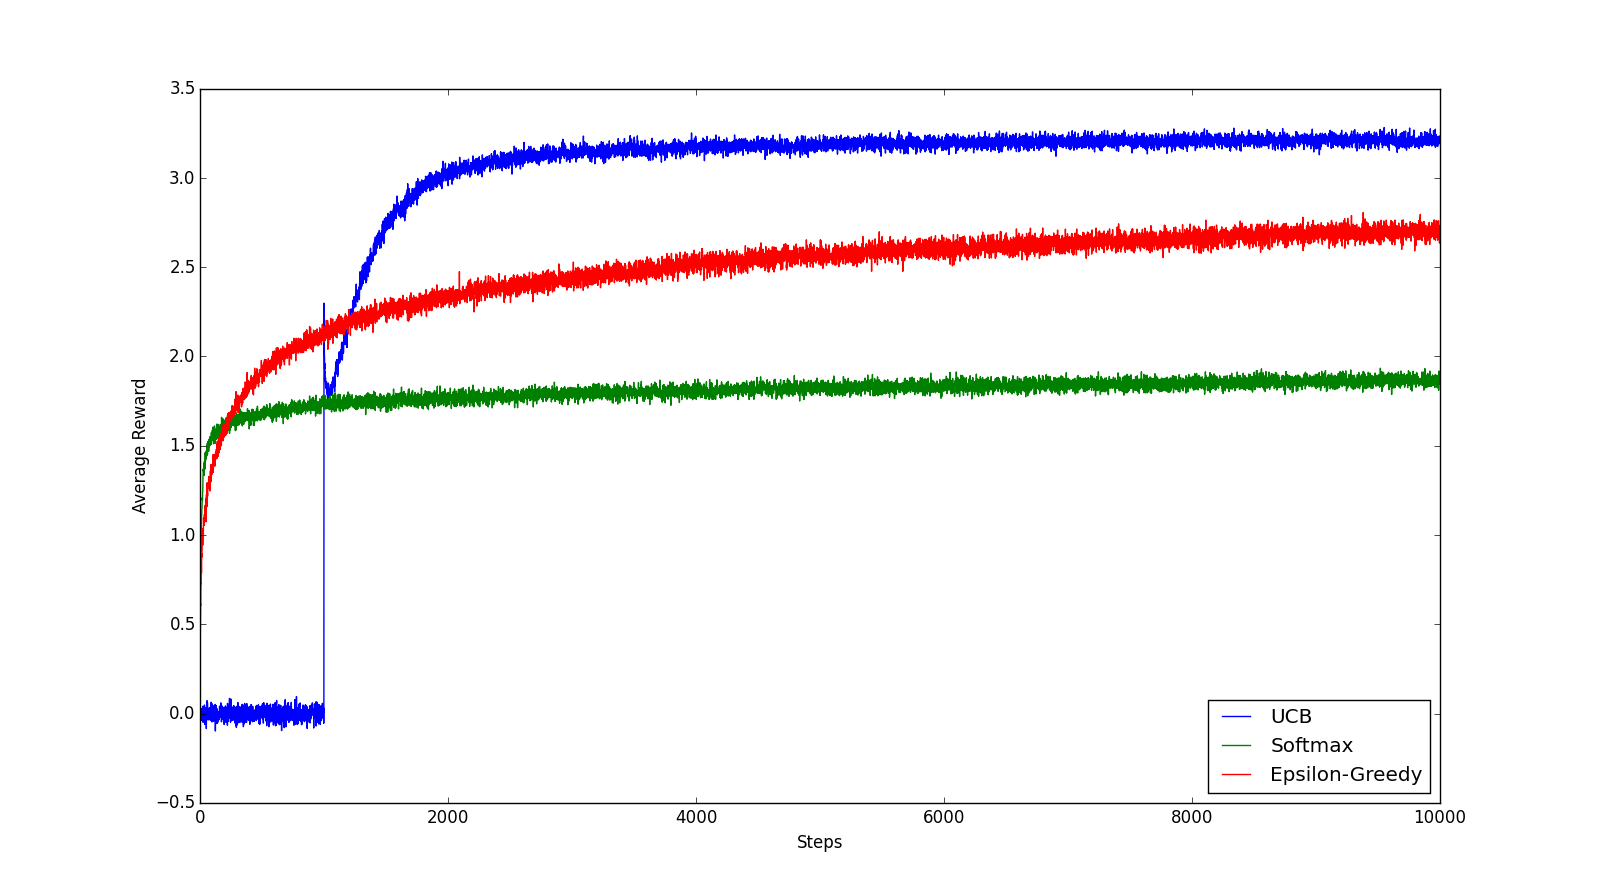
\includegraphics[width=\linewidth]{compare_ucb_1000_arms_10000_steps_average_reward.png}
  \caption{Plot comparing the average reward accrued using UCB, $\epsilon$-greedy and Softmax Action Selection on the 1000-armed testbed over 10000 timesteps. These data are averaged over 2000 runs of different bandit problems. For $\epsilon$-greedy approach, $\epsilon = 0.1 $ and for softmax action selection, $\tau = 0.1$ where $\tau$ is the temperature parameter.}
  \label{fig:eg1}
\end{figure}

\begin{figure}[H]
  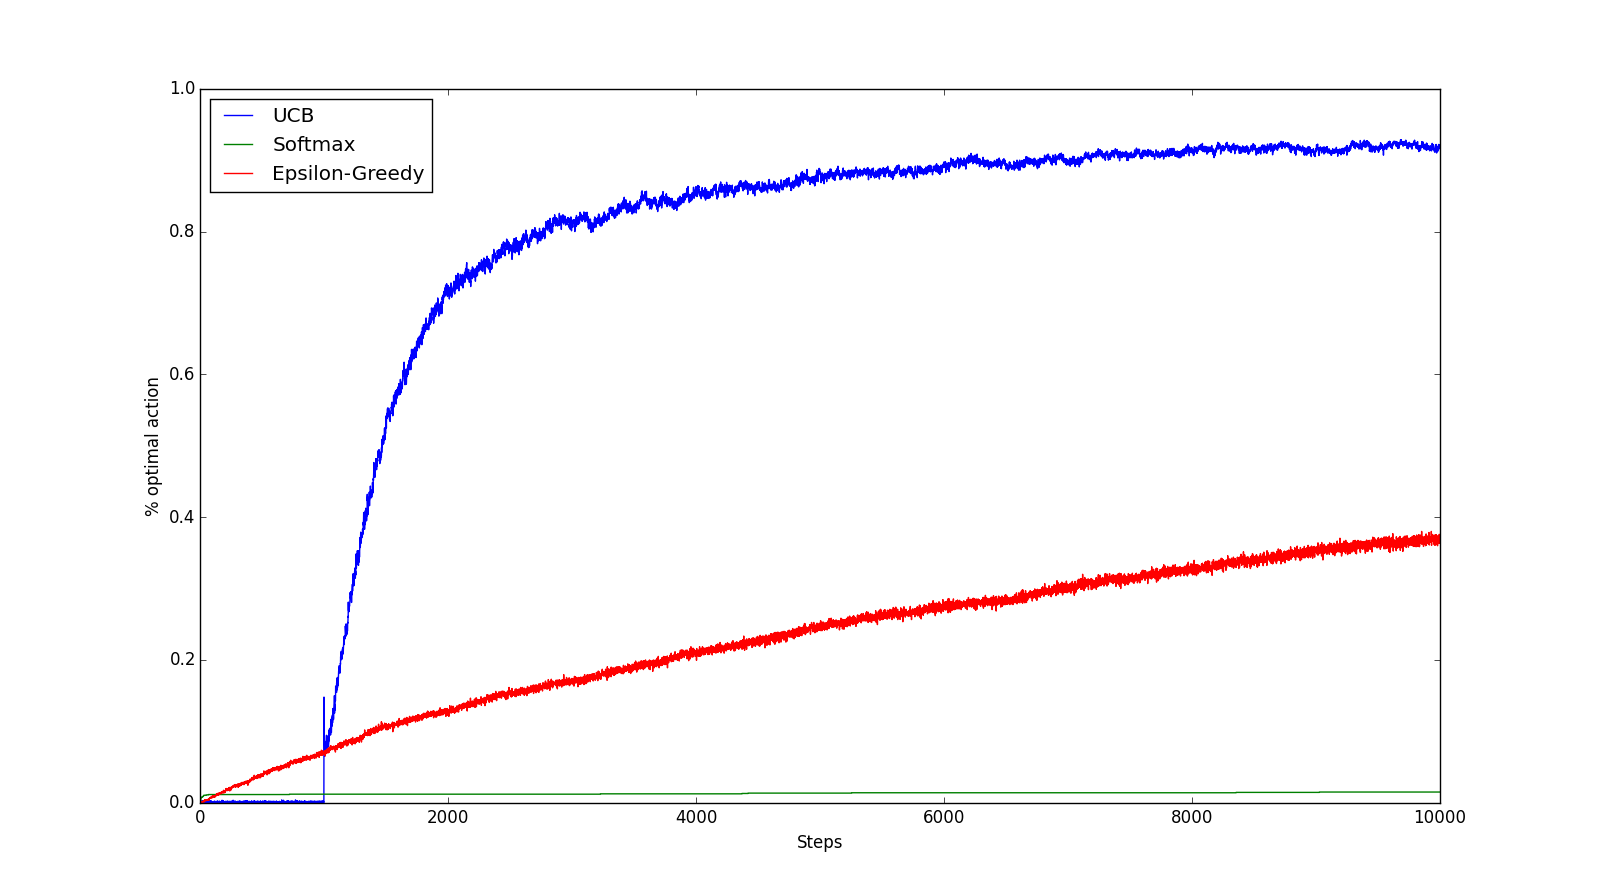
\includegraphics[width=\linewidth]{compare_ucb_1000_arms_10000_steps_optimal_action.png}
  \caption{Plot comparing the average reward accrued using UCB, $\epsilon$-greedy and Softmax Action Selection on the 1000-armed testbed over 10000 timesteps. These data are averaged over 2000 runs of different bandit problems. For $\epsilon$-greedy approach, $\epsilon = 0.1 $ and for softmax action selection, $\tau = 0.1$ where $\tau$ is the temperature parameter.}
  \label{fig:eg1}
\end{figure}

\subsubsection{Plots for 20000 time-steps}
\begin{figure}[H]
  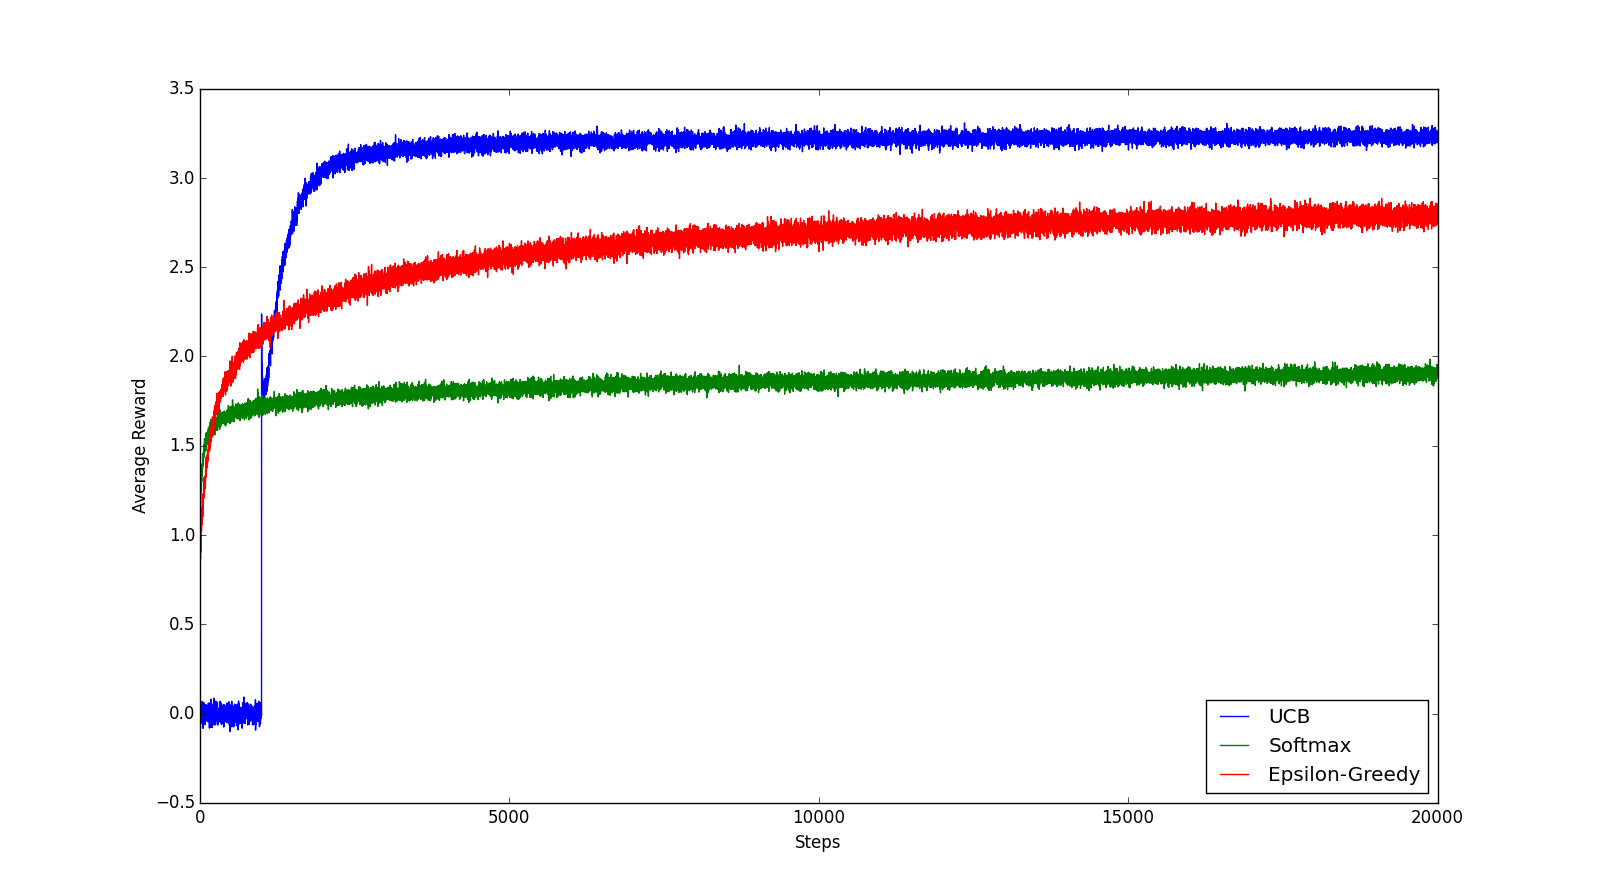
\includegraphics[width=\linewidth]{compare_ucb_1000_arms_20000_steps_average_reward.png}
  \caption{Plot comparing the average reward accrued using UCB, $\epsilon$-greedy and Softmax Action Selection on the 1000-armed testbed over 20000 timesteps. These data are averaged over 2000 runs of different bandit problems. For $\epsilon$-greedy approach, $\epsilon = 0.1 $ and for softmax action selection, $\tau = 0.1$ where $\tau$ is the temperature parameter.}
  \label{fig:eg1}
\end{figure}

\begin{figure}[H]
  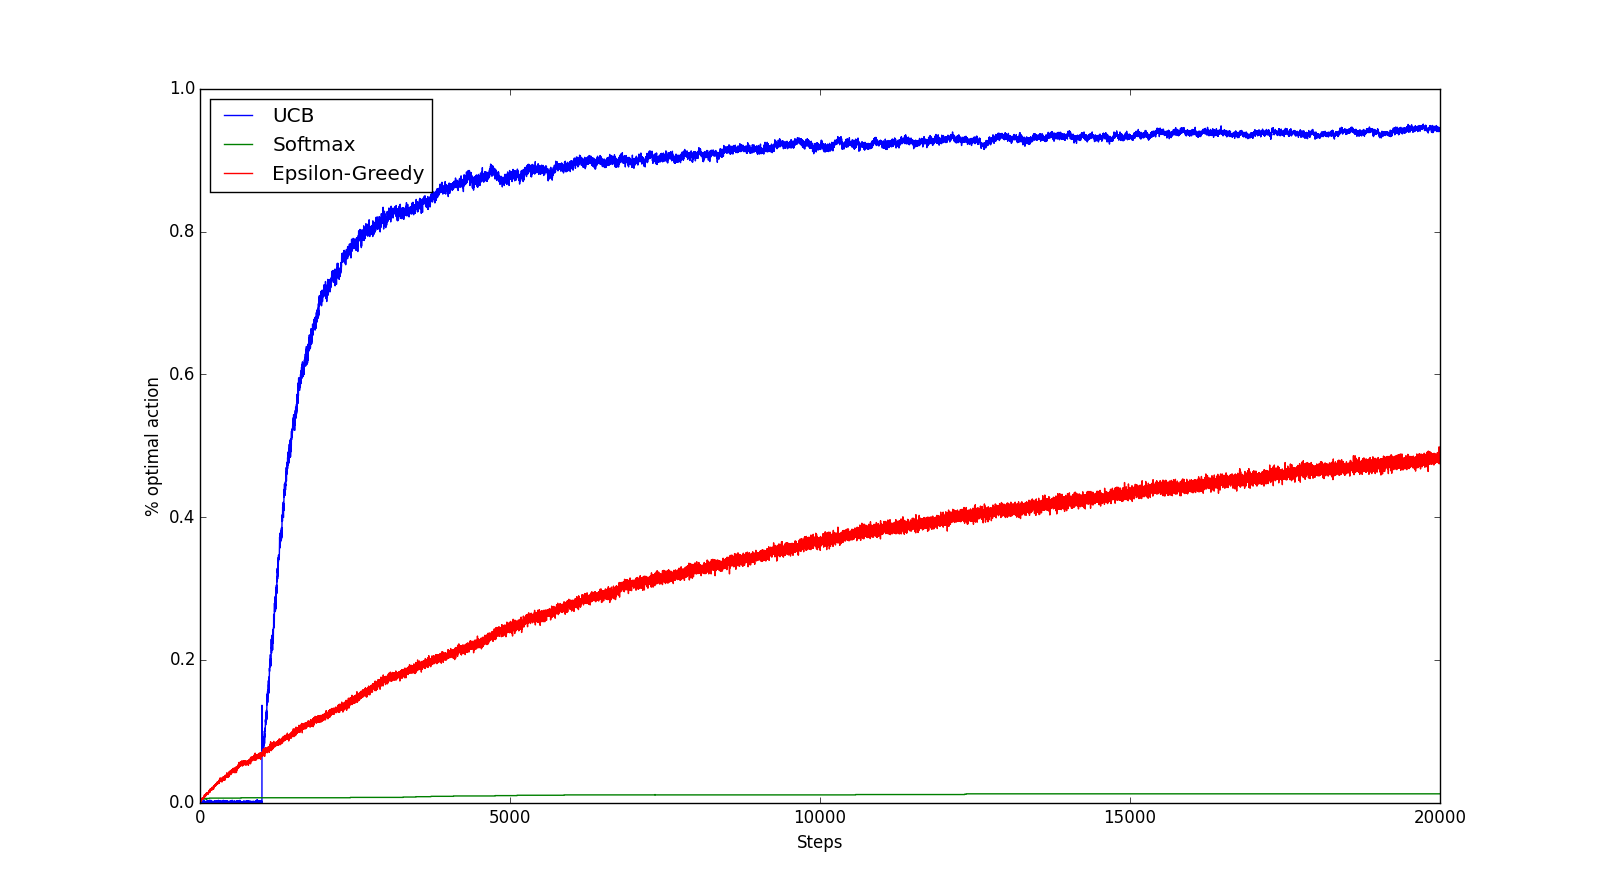
\includegraphics[width=\linewidth]{compare_ucb_1000_arms_20000_steps_optimal_action.png}
  \caption{Plot comparing the average reward accrued using UCB, $\epsilon$-greedy and Softmax Action Selection on the 1000-armed testbed over 20000 timesteps. These data are averaged over 2000 runs of different bandit problems. For $\epsilon$-greedy approach, $\epsilon = 0.1 $ and for softmax action selection, $\tau = 0.1$ where $\tau$ is the temperature parameter.}
  \label{fig:eg1}
\end{figure}

\section{Analysis of the Plots}
\subsection{Plots for $\epsilon$-greedy action selection for 10 arms}
The simulation for $\epsilon$-greedy action selection is run on a 10-armed bandit testbed for three different values of $\epsilon$ which are 0.0 (greedy) , 0.1 (being greedy 90 \% of the time) , 0.01 (being greedy 99 \% of the time). We can notice in the plot of these simulations that over a time-step of 1000, $\epsilon = 0.1$ does the best both in terms of average reward and \% optimal action selection. Notice that in the long run $\epsilon = 0.01$ might do better than $\epsilon = 0.1$ both in terms of average reward and \% optimal action selection. The greedy method ($\epsilon = 0.0$) performs significantly worse in the long run because it often gets stuck performing a suboptimal action. The \% optimal action selection shows that the greedy action selection found the optimal action in only approximately one-third of the tasks. Therefore in two-third of the tasks,its initial samples of optimal action were bad and it never returned to them. In comparison to greedy, $\epsilon$-greedy perform better because they continue to explore and improve their chance of recognizing the optimal action.

\subsection{Plots for Softmax Action Selection for 10 arms}
The simulation for softmax action selection is run on a 10-armed bandit testbed for four different values of temperature which are 0.01, 0.1, 1 and 10. We can notice in the plot of these simulations that over a time-step of 1000, temperature of 0.1 does the best both in terms of average reward and \% optimal action selection. We can notice that if the value of temperature is too low (ie 0.01), we essentially end up behaving greedily but it often gets stuck performing a suboptimal action. Similarly we can also notice that if the value of temperature is too high (ie 10), we essentially end up being random in our action selection and perform badly and hence \% optimal action is only 10\% ie we are picking up the optimal arm uniformly randomly. We can notice that temperature value of 0.1 is the most apt as it carefully balances exploration and exploitation. Also this is the only temperature which continues to grow for both the plots while the other temperatures seem to saturate out.

\subsection{Plots for UCB vs $\epsilon$-greedy vs Softmax Action Selection for 10 arms}
The simulation for comparison of UCB with other action selection plots is run on a 10-armed bandit testbed for $\epsilon=0.1$ for $\epsilon$-greedy and temperature = 0.1 for softmax action selection over a 1000 timesteps. We can clearly notice that UCB does the best both in terms of average reward and \% optimal action selection. Initially, UCB performs bad but that can be attributed to the fact that initially UCB plays all the onces once and is forced to take suboptimal actions. Also in comparison $\epsilon$-greedy performs better that softmax action selection for this particular choice of $\epsilon$ and temperature. But we can conclude that UCB performs the best in case of 10 arms over 1000 timesteps.

\subsection{Plots for UCB vs $\epsilon$-greedy vs Softmax Action Selection for 1000 arms}
Now we do the comparison of algorithms as the number of arms increase. We increase the number of arms from 10 to 1000 and compare the algorithms for different values of time-steps.
\subsubsection{Plots for 1000 timesteps}
If we keep the number of timesteps the same as the one in the previous question, we can notice that UCB performs the worst in comparison to $\epsilon$-greedy and softmax action selection. $\epsilon$-greedy performs the best eventually(ie in 1000 timesteps) because it starts picking up sub-optimal action which still does better than UCB because UCB is continuing to play each arm one and hence doesn't repeatedly take a sub-optimal action. In the $\epsilon$-greedy action selection doesn't visit all the arms and selects action from a set of few sampled arms. It is not fair to compare $\epsilon$-greedy and softmax action selection amongst themselves as these are parameterized by $\epsilon$ and temperature and hence for different values of $\epsilon$ and temperature may yield different results but this is sufficient to conclude that both $\epsilon$-greedy and softmax action selection perform better than UCB for 1000 time-steps simply because UCB continues to play each arm once while $\epsilon$-greedy and softmax action selection behave greedily majority of the time. This can also be seen from the \%optimal action plot which shows that UCB selects optimal action once in 1000 times which should be expected. This is also not fair on UCB and hence in the next analysis we increase the time step from 1000 to 10000 and 20000.

\subsubsection{Plots for 10000 timesteps}
As we increase the number of timesteps from 1000 to 10000 we can immediately see that UCB performs best in comparison to $\epsilon$-greedy and softmax action selection. Initially again, UCB performs the worst but that can again be attributed to the fact that UCB is playing each arm once. We can also see that there is sudden shoot in average reward after 1000 steps which can be attributed to the fact that UCB now starts being greedy with respect to the upper confidence bound on the estimates. Again we see that $\epsilon$-greedy does better than softmax action selection which is not a fair comparison as they are parameterised by $\epsilon$ and temperature.

\subsubsection{Plots for 20000 timesteps}
The results for 20000 timesteps are similar to the ones for 10000 timesteps. One thing to notice though is that $\epsilon$-greedy seems to be converging to UCB in terms of average reward and \% optimal action selection.

\section{Conclusion}
\begin{itemize}
	\item $\epsilon$-greedy T = 1000 and N = 10 
	\begin{itemize}
		\item maximum average reward is obtained for $\epsilon$ = 0.1
		\item maximum optimal action is obtained for $\epsilon$ = 0.1
	\end{itemize}
	\item softmax action selection T = 1000 and N = 10
	\begin{itemize}
		\item maximum average reward is obtained for temperature = 0.1
		\item maximum optimal action is obtained for temperature = 0.1
	\end{itemize}
	\item UCB vs $\epsilon$-greedy vs softmax action selection T = 1000 and N = 10
	\begin{itemize}
		\item maximum average reward is obtained for UCB
		\item maximum optimal action is obtained for UCB
	\end{itemize}
	\item UCB vs $\epsilon$-greedy vs softmax action selection T = 1000 and N = 1000
	\begin{itemize}
		\item maximum average reward is obtained for $\epsilon$-greedy with $\epsilon = 0.1$
		\item maximum optimal action is obtained for $\epsilon$-greedy with $\epsilon = 0.1$
	\end{itemize}
	\item UCB vs $\epsilon$-greedy vs softmax action selection T = 10000 and N = 1000
	\begin{itemize}
		\item maximum average reward is obtained for UCB
		\item maximum optimal action is obtained for UCB
	\end{itemize}
	\item UCB vs $\epsilon$-greedy vs softmax action selection T = 20000 and N = 1000
	\begin{itemize}
		\item maximum average reward is obtained for UCB
		\item maximum optimal action is obtained for UCB
	\end{itemize}
\end{itemize}

\section{Code Listing}
\subsection{Bandit Class for object instantiation}
\lstinputlisting[language=Python]{../bandit.py}
\subsection{Python Library for Simulating the Bandit Problem}
\lstinputlisting[language=Python]{../simulateBandit.py}
\subsection{Python Script to Generate Plots for $\epsilon$-greedy action selection}
\lstinputlisting[language=Python]{../epsilonGreedy.py}
\subsection{Python Script to Generate Plots for softmax action selection}
\lstinputlisting[language=Python]{../softmax.py}
\subsection{Python Script to Generate Plots for comparing UCB vs $\epsilon$-greedy action selection vs softmax action selection}
\lstinputlisting[language=Python]{../ucb.py}
\end{document}
